\documentclass{beamer}

\usetheme{Madrid}
\usecolortheme{default}

\usepackage[italian]{babel}
\usepackage[utf8]{inputenc}
\usepackage[T1]{fontenc}
\usepackage{xcolor}
\usepackage{verbatim}
\usepackage{tikz}
\usepackage{listings}
\usetikzlibrary{shapes.geometric, arrows, positioning}

\lstset{
    language=SQL,
    basicstyle=\ttfamily\small,
    keywordstyle=\color{blue},
    commentstyle=\color{gray},
    stringstyle=\color{darkgray},
    breaklines=true,
    showstringspaces=false
}

\title{Basi di Dati}
\subtitle{SQL DQL -- Interrogare i dati}
\author{Prof. Federico Mazzini}
\institute{I.I.S. Francesco Alberghetti}
\date{A.S. 2025 -- 2026}

\begin{document}

%==============================================================================
\begin{frame}
\titlepage
\end{frame}

%==============================================================================
\section{Dal database ai dati}

%==============================================================================
\begin{frame}{Data Query Language (DQL)}
Un database non serve solo a memorizzare dati.

\medskip
Serve a \textbf{interrogarli}, analizzarli, estrarne informazione:

\begin{itemize}
    \item Quali studenti hanno media sopra 8?
    \item Quanti ordini ha fatto un cliente?
    \item Qual è il totale delle vendite?
\end{itemize}

\end{frame}

%==============================================================================
\section{SQL e DQL}
%==============================================================================

\begin{frame}{Cos'è il DQL}
\begin{block}{Definizione}
Il DQL (Data Query Language) è la parte di SQL che permette di \textbf{interrogare i dati} presenti nelle tabelle.
\end{block}

\medskip
Il comando fondamentale del DQL è:

\begin{center}
\Large \texttt{SELECT}
\end{center}

\medskip
Con SELECT possiamo estrarre informazioni dal database.
\end{frame}

%==============================================================================
\begin{frame}[fragile]{La struttura base di SELECT}
La forma generale è:

\begin{lstlisting}[language=SQL]
SELECT attributi
FROM tabella
WHERE condizione;
\end{lstlisting}

\begin{itemize}
    \item \textbf{SELECT} → cosa vogliamo vedere
    \item \textbf{FROM} → da quale tabella
    \item \textbf{WHERE} → con quali condizioni
\end{itemize}
\end{frame}

%==============================================================================
\begin{frame}[fragile]{SELECT}

\begin{lstlisting}[language=SQL]
SELECT nome, cognome
FROM studenti;
\end{lstlisting}

\medskip
\textbf{Risultato:}
\begin{center}
\begin{tabular}{|l|l|}
\hline
Nome & Cognome \\
\hline
Luca & Rossi \\
Anna & Bianchi \\
Paolo & Verdi \\
\hline
\end{tabular}
\end{center}

\end{frame}

%==============================================================================
\begin{frame}[fragile]{SELECT *}

Utilizzando l'asterisco, vengono selezionate tutte le colonne, senza bisogno di specificarne singolarmente.

\begin{lstlisting}[language=SQL]
SELECT *
FROM studenti;
\end{lstlisting}

\medskip
\textbf{Risultato:}
\begin{center}
\begin{tabular}{|l|l|l|l|l|}
\hline
id\_studente & Matricola & Nome & Cognome & Data\_nascita \\
\hline
1 & 1001 & Luca & Rossi & 2007-03-15 \\
2 & 1002 & Anna & Bianchi & 2007-07-21 \\
3 & 1003 & Paolo & Verdi & 2006-11-03 \\
\hline
\end{tabular}
\end{center}

\medskip
In tabelle con molte colonne, utilizzare ''*'' rende difficile la lettura dei risultati.
\end{frame}

%==============================================================================
\begin{frame}[fragile]{SELECT con Alias}
\small
E' possibile utilizzare un alias per il nome delle colonne.

\begin{lstlisting}[language=SQL]
SELECT nome AS Nome Studente, 
       cognome AS Cognome Studente
FROM studenti;
\end{lstlisting}

\medskip
\textbf{Risultato:}
\begin{center}
\begin{tabular}{|c|c|}
\hline
Nome Studente & Cognome Studente \\
\hline
Luca & Rossi \\
Anna & Bianchi \\
Paolo & Verdi \\
\hline
\end{tabular}
\end{center}

\medskip
\begin{itemize}
    \item Semplifica la lettura dei risultati nel caso di tabelle con nomi tecnici e poco parlanti
    \item Non modifica il nome delle colonne, solo la loro visualizzazione nella specifica SELECT
\end{itemize}
\end{frame}


%==============================================================================
\begin{frame}[fragile]{WHERE}
E' possibile filtrare i risultati della SELECT utilizzando la clausola WHERE. 

\bigskip
\textbf{Esempio} trovare lo studente con ID 3:

\begin{lstlisting}[language=SQL]
SELECT nome, cognome, data_nascita
FROM studenti
WHERE id_studente = 3;
\end{lstlisting}

\end{frame}

%==============================================================================
\begin{frame}[fragile]{WHERE}
E' possibile filtrare i risultati della SELECT utilizzando la clausola WHERE. 

\bigskip
\textbf{Esempio} tutti gli studenti nati dopo il 2006:

\begin{lstlisting}[language=SQL]
SELECT nome, cognome, data_nascita
FROM studenti
WHERE data_nascita > '2006-12-31';
\end{lstlisting}

\end{frame}

%==============================================================================
\begin{frame}[fragile]{WHERE e condizioni logiche}
La clausola WHERE restituisce tutte le righe che soddisfano la condizione logica. 
Infatti, utilizzando la seguenti condizioni:
\bigskip

\textbf{Restituisce tutti gli studenti}
\begin{lstlisting}[language=SQL]
SELECT nome, cognome
FROM studenti
WHERE 1 = 1;
\end{lstlisting}

\bigskip
\textbf{Restituisce nessuno studente}
\begin{lstlisting}[language=SQL]
SELECT nome, cognome
FROM studenti
WHERE 1 = 0;
\end{lstlisting}

\end{frame}

%==============================================================================
\begin{frame}[fragile]{WHERE e operatori di confronto}
Gli operatori di confronto servono a definire condizioni puntuali o basate su valori:

\begin{itemize}
    \item =,  >, <, >=, <=, <> (diverso), LIKE
\end{itemize}

\medskip
Esempio: selezionare studenti nati dopo il 31/12/2006

\begin{lstlisting}[language=SQL]
SELECT nome, cognome
FROM studenti
WHERE data_nascita > '2006-12-31';
\end{lstlisting}
\end{frame}


%==============================================================================
\begin{frame}[fragile]{WHERE e operatori di confronto}
Il LIKE permette di filtrare stringhe secondo un pattern lessicale.

\medskip 

E' possibile esprimere condizioni come le seguenti:

\bigskip
\textbf{\textit{Studenti il cui cognome inizia con "R"}}
\begin{lstlisting}[language=SQL]
SELECT nome, cognome
FROM studenti
WHERE cognome LIKE 'R%';
\end{lstlisting}

\bigskip
\textbf{\textit{Studenti il cui nome contiene "an"}}
\begin{lstlisting}[language=SQL]
SELECT nome, cognome
FROM studenti
WHERE nome LIKE '%an%';
\end{lstlisting}

\end{frame}

%==============================================================================
\begin{frame}[fragile]{WHERE e operatori logici}
Gli operatori logici servono a combinare più condizioni:

\begin{itemize}
    \item AND → entrambe le condizioni devono essere vere
    \item OR → almeno una condizione deve essere vera
    \item NOT → nega la condizione
\end{itemize}


\begin{lstlisting}[language=SQL]
SELECT nome, cognome
FROM studenti
WHERE data_nascita > '2006-12-31' AND
      classe = '5A';
\end{lstlisting}
\end{frame}

%==============================================================================
\begin{frame}[fragile]{WHERE e operatori logici}
Gli operatori logici servono a combinare più condizioni:

\begin{itemize}
    \item AND → entrambe le condizioni devono essere vere
    \item OR → almeno una condizione deve essere vera
    \item NOT → nega la condizione
\end{itemize}


\begin{lstlisting}[language=SQL]
SELECT nome, cognome
FROM studenti
WHERE classe = '5A' OR
      classe = '5B';
\end{lstlisting}

\end{frame}

%==============================================================================
\begin{frame}[fragile]{WHERE e operatori logici}
Gli operatori logici servono a combinare più condizioni:

\begin{itemize}
    \item AND → entrambe le condizioni devono essere vere
    \item OR → almeno una condizione deve essere vera
    \item NOT → nega la condizione
\end{itemize}

\begin{lstlisting}[language=SQL]
SELECT nome, cognome
FROM studenti
WHERE NOT classe = '5A';
\end{lstlisting}
\end{frame}


%==============================================================================
\begin{frame}[fragile]{WHERE e combinazioni più complesse}
Attenzione alla concatenazione degli operatori logici. Le seguenti query, sono diverse:

\begin{lstlisting}[language=SQL]
SELECT nome, cognome
FROM studenti
WHERE (classe = '5A' OR classe = '5B')
      AND cognome LIKE 'R%';
\end{lstlisting}

\begin{lstlisting}[language=SQL]
SELECT nome, cognome
FROM studenti
WHERE classe = '5A' OR classe = '5B'
      AND cognome LIKE 'R%';
\end{lstlisting}

\end{frame}

%==============================================================================
\begin{frame}[fragile]{Ordinare i risultati}
Esempio: ordinare gli studenti per cognome in ordine alfabetico:

\begin{lstlisting}[language=SQL]
SELECT nome, cognome, matricola
FROM studenti
ORDER BY cognome ASC;
\end{lstlisting}

\medskip
\begin{itemize}
    \item ASC → ordine crescente
    \item DESC → ordine decrescente
\end{itemize}
\end{frame}





%%========================== FUNZIONI DI AGGREGAZIONE ==========================
%%==============================================================================

\begin{frame}[fragile]{Aggregare i dati}
Si consideri la tabella \textbf{verifiche} contenente i seguenti record:

\begin{center}
\begin{tabular}{|c|c|c|}
\hline
\textbf{id\_studente} & \textbf{materia} & \textbf{voto} \\ \hline
1 & Informatica & 8 \\ \hline
2 & Informatica & 5 \\ \hline
3 & Informatica & NULL \\ \hline
4 & Informatica & 10 \\ \hline
5 & Informatica & 7 \\ \hline
\end{tabular}
\end{center}

\medskip
\textbf{Obiettivo:} Determinare il numero di studenti che hanno sostenuto la verifica, il voto massimo registrato e la media dei voti della classe.
\end{frame}

%%==============================================================================
\begin{frame}[fragile]{Aggregare i dati}
Viene riportata di seguito la query di aggregazione necessaria:

\begin{lstlisting}[language=SQL]
SELECT 
    COUNT(voto) AS num_verifiche,
    MAX(voto) AS voto_max,
    AVG(voto) AS media_voti
FROM verifiche;
\end{lstlisting}

\textbf{Risultato ottenuto:}
\begin{center}
\begin{tabular}{|c|c|c|}
\hline
\textbf{num\_verifiche} & \textbf{voto\_max} & \textbf{media\_voti} \\ \hline
4 & 10 & 7.5 \\ \hline
\end{tabular}
\end{center}

\begin{itemize}
    \item Il sistema elabora i 5 record di partenza restituendo \textbf{un'unica riga} sintetica.
    \item Il valore \texttt{NULL} viene ignorato sia nel conteggio (\texttt{COUNT}) che nel calcolo della media (\texttt{AVG}).
\end{itemize}
\end{frame}

%%==============================================================================
\begin{frame}[fragile]{Aggregare i dati - Definizione}
Le funzioni di aggregazione operano su un \textbf{insieme di righe} (set di dati) e restituiscono un \textbf{unico valore} riassuntivo.

\begin{itemize}
    \item \texttt{COUNT(*)}: Conteggio di tutte le righe (inclusi i valori NULL).
    \item \texttt{SUM(colonna)}: Somma dei valori numerici della colonna specificata.
    \item \texttt{AVG(colonna)}: Calcolo della media aritmetica dei valori.
    \item \texttt{MIN() / MAX()}: Individuazione dei valori estremi (applicabile a numeri, date e stringhe).
\end{itemize}

\end{frame}

%%==============================================================================
\begin{frame}[fragile]{Aggregare i dati - Utilizzo dell'alias}
Ha sempre senso utilizzare un alias con le funzioni di aggregazione per rendere più esplicita la query

\begin{lstlisting}[language=SQL]
-- Calcolo della media generale dei voti
SELECT AVG(voto) AS media_generale
FROM verifiche;

-- Statistiche descrittive
SELECT 
    COUNT(voto) AS totale_voti,
    SUM(voto)   AS somma_voti,
    MIN(voto)   AS voto_minimo,
    MAX(voto)   AS voto_massimo
FROM verifiche;
\end{lstlisting}

\end{frame}


%%==============================================================================
\begin{frame}[fragile]{Aggregare i dati - Criterio specifico}
Si consideri la necessità di visualizzare la media dei voti accanto al nome di ogni materia:

\begin{center}
\begin{tabular}{|c|c|c|}
\hline
\textbf{id} & \textbf{materia} & \textbf{voto} \\ \hline
1 & Informatica & 8 \\ \hline
2 & Matematica  & 10 \\ \hline
3 & Informatica & 7 \\ \hline
4 & Matematica  & 6 \\ \hline
\end{tabular}
\end{center}

\medskip
\begin{lstlisting}[language=SQL]
SELECT materia, AVG(voto) 
FROM verifiche;
\end{lstlisting}

\end{frame}


%%==============================================================================
\begin{frame}[fragile]{Aggregare i dati - Criterio specifico}
Si consideri la necessità di visualizzare la media dei voti accanto al nome di ogni materia:

\begin{center}
\begin{tabular}{|c|c|c|}
\hline
\textbf{id} & \textbf{materia} & \textbf{voto} \\ \hline
1 & Informatica & 8 \\ \hline
2 & Matematica  & 10 \\ \hline
3 & Informatica & 7 \\ \hline
4 & Matematica  & 6 \\ \hline
\end{tabular}
\end{center}

\medskip
\begin{lstlisting}[language=SQL]
SELECT materia, AVG(voto) 
FROM verifiche;
\end{lstlisting}

\begin{alertblock}{Errore!}
La query genera un errore o un risultato errato: non è possibile mostrare più righe per la colonna \texttt{materia} e una sola riga per la media (\texttt{AVG}). Il sistema richiede un \textbf{criterio di raggruppamento}.
\end{alertblock}
\end{frame}

%%==============================================================================
\begin{frame}[fragile]{Specificare il Criterio: GROUP BY}
Si consideri la necessità di visualizzare la media dei voti accanto al nome di ogni materia:

\begin{center}
\begin{tabular}{|c|c|c|}
\hline
\textbf{id} & \textbf{materia} & \textbf{voto} \\ \hline
1 & Informatica & 8 \\ \hline
2 & Matematica  & 10 \\ \hline
3 & Informatica & 7 \\ \hline
4 & Matematica  & 6 \\ \hline
\end{tabular}
\end{center}

\begin{lstlisting}[language=SQL]
SELECT materia, AVG(voto) AS media_materia
FROM verifiche
GROUP BY materia;
\end{lstlisting}

\end{frame}

%%==============================================================================
\begin{frame}[fragile]{Specificare il Criterio: GROUP BY}
Si consideri la necessità di visualizzare la media dei voti accanto al nome di ogni materia:

\begin{center}
\begin{tabular}{|c|c|c|}
\hline
\textbf{id} & \textbf{materia} & \textbf{voto} \\ \hline
1 & Informatica & 8 \\ \hline
2 & Matematica  & 10 \\ \hline
3 & Informatica & 7 \\ \hline
4 & Matematica  & 6 \\ \hline
\end{tabular}
\end{center}

\begin{lstlisting}[language=SQL]
SELECT materia, AVG(voto) AS media_materia
FROM verifiche
GROUP BY materia;
\end{lstlisting}

\textbf{Risultato dell'operazione:}
\begin{center}
\begin{tabular}{|c|c|}
\hline
\textbf{materia} & \textbf{media\_materia} \\ \hline
Informatica & 7.5 \\ \hline
Matematica  & 8.0 \\ \hline
\end{tabular}
\end{center}

\end{frame}


%%==============================================================================
\begin{frame}[fragile]{Raggruppare i Dati: GROUP BY}
Il costrutto \texttt{GROUP BY} opera secondo la logica di \textbf{Split, Apply, Combine}.

\begin{enumerate}
    \item \textbf{Split}: I record vengono divisi in gruppi in base alla colonna specificata.
    \item \textbf{Apply}: La funzione di aggregazione viene calcolata per ogni gruppo.
    \item \textbf{Combine}: I risultati parziali vengono uniti in una tabella di sintesi.
\end{enumerate}

\vspace{0.3cm}
\begin{center}
    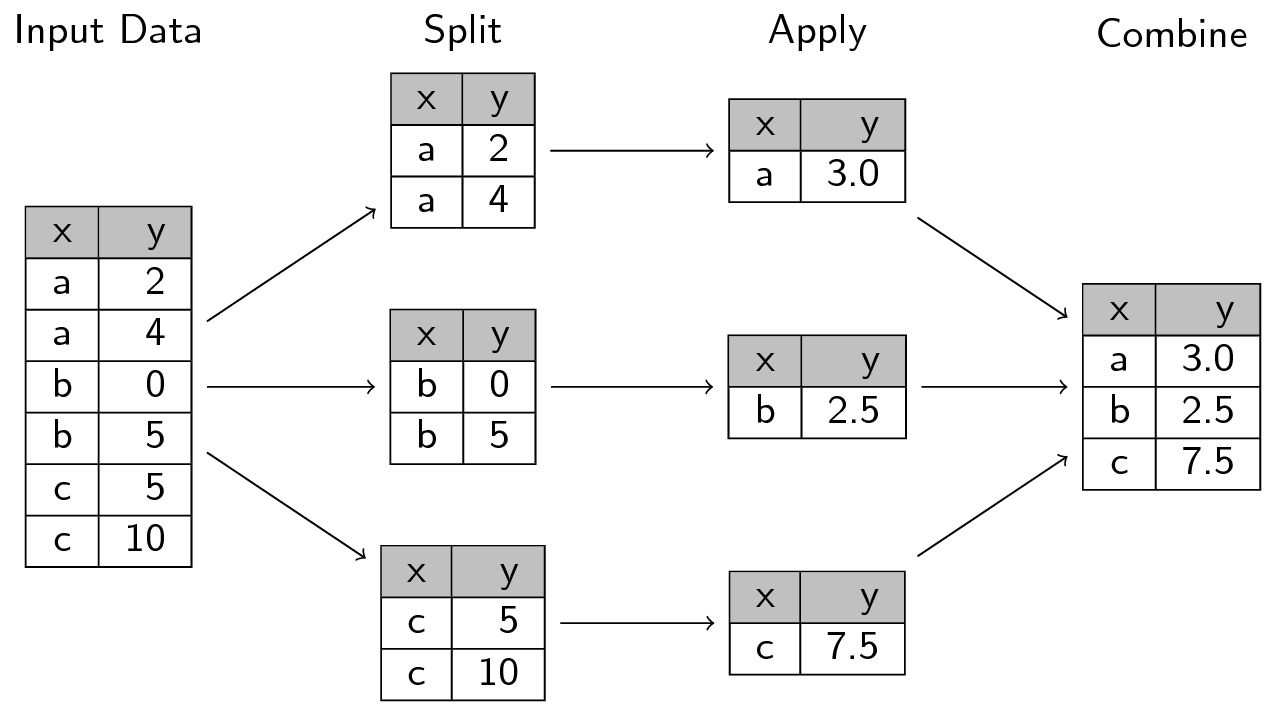
\includegraphics[width=0.9\linewidth, height=3.5cm, keepaspectratio]{images/split-apply-combine.png}
\end{center}
\vspace{0.3cm}

\end{frame}

%%==============================================================================
\begin{frame}[fragile]{Raggruppare i Dati: GROUP BY}

\textbf{Regola pratica} 

Ogni colonna presente nella \texttt{SELECT} che non sia una funzione di aggregazione \textbf{deve} essere inclusa nel \texttt{GROUP BY}.

\vspace{0.3cm}
\begin{center}
    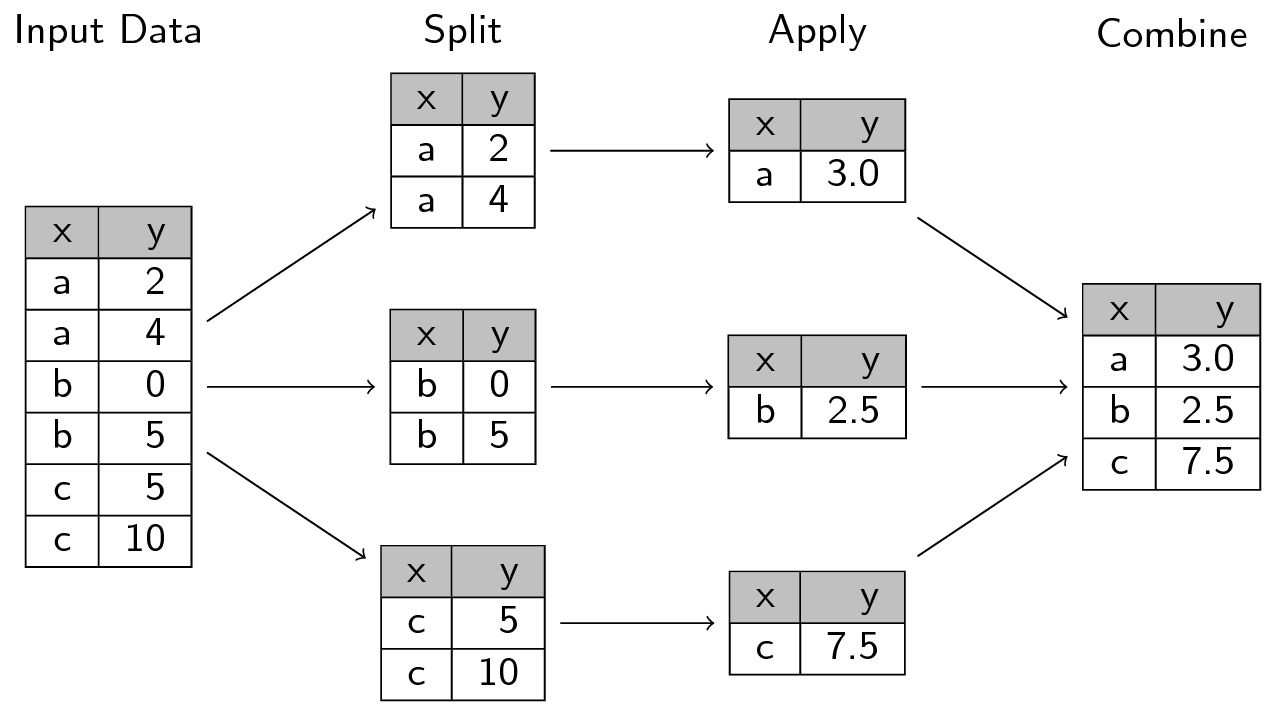
\includegraphics[width=0.9\linewidth, height=3.5cm, keepaspectratio]{images/split-apply-combine.png}
\end{center}
\vspace{0.3cm}

\end{frame}

%%==============================================================================
\begin{frame}[fragile]{Il Problema: Filtrare i Risultati Aggregati}
Si ipotizzi di voler individuare le materie la cui media dei voti è superiore a 8.

\medskip
\textbf{Tentativo errato con WHERE:}
\begin{lstlisting}[language=SQL]
SELECT materia, AVG(voto) AS media
FROM verifiche
WHERE voto > 8
GROUP BY materia;
\end{lstlisting}

\begin{alertblock}{Analisi dell'errore}
La clausola \texttt{WHERE} agisce \textbf{prima} del calcolo della media. La query sopra citata scarterebbe tutti i voti inferiori o uguali a 8 \textit{prima} di raggruppare, calcolando quindi la media solo sui voti eccellenti. Il risultato non sarebbe la "media della materia", ma la "media dei soli voti alti".
\end{alertblock}
\end{frame}

%%==============================================================================
\begin{frame}[fragile]{La Soluzione: Clausola HAVING}
Per filtrare i risultati prodotti dalle funzioni di aggregazione (\texttt{AVG, SUM, COUNT}, ecc.), è necessario utilizzare la clausola \textbf{\texttt{HAVING}}.

\medskip
Questa clausola permette di applicare una condizione di ricerca a gruppi di righe o ad aggregati, agendo logicamente \textbf{dopo} il raggruppamento dei dati.

\begin{lstlisting}[language=SQL]
SELECT materia, AVG(voto) AS media
FROM verifiche
GROUP BY materia
HAVING AVG(voto) > 8;
\end{lstlisting}

\begin{exampleblock}{Logica Operativa}
Mentre il \texttt{WHERE} definisce quali record atomici partecipano al calcolo, l'\texttt{HAVING} definisce quali gruppi risultanti devono essere visualizzati nel report finale.
\end{exampleblock}
\end{frame}

%%==============================================================================
\begin{frame}[fragile]{Ordine di Esecuzione e Flusso Dati}
L'ordine logico con cui il DBMS processa la query chiarisce la distinzione tra i due filtri:

\begin{center}
\begin{tabular}{|l|l|l|}
\hline
\textbf{Ordine} & \textbf{Clausola} & \textbf{Azione} \\ \hline
1 & \texttt{FROM / JOIN} & Identificazione delle tabelle \\ \hline
2 & \textbf{\texttt{WHERE}} & \textbf{Filtro sulle righe originali} \\ \hline
3 & \texttt{GROUP BY} & Formazione dei gruppi \\ \hline
4 & \textbf{\texttt{HAVING}} & \textbf{Filtro sui gruppi prodotti} \\ \hline
5 & \texttt{SELECT} & Proiezione delle colonne e calcoli \\ \hline
6 & \texttt{ORDER BY} & Ordinamento finale \\ \hline
\end{tabular}
\end{center}

\medskip
\textbf{Nota:} Poiché l'\texttt{HAVING} viene valutato dopo il \texttt{GROUP BY}, è possibile utilizzarvi le funzioni di aggregazione, operazione vietata all'interno del \texttt{WHERE}.
\end{frame}

%%==============================================================================
\begin{frame}[fragile]{Casi d'Uso: Filtrare sul Conteggio (COUNT)}
L'\texttt{HAVING} risulta fondamentale per analisi statistiche basate sulla numerosità dei gruppi.

\medskip
\textbf{Esempio:}
\begin{lstlisting}[language=SQL]
SELECT classe, COUNT(id_studente) AS numero_studenti
FROM studenti
GROUP BY classe
HAVING COUNT(id_studente) > 20;
\end{lstlisting}

\begin{itemize}
    \item Il \texttt{GROUP BY} crea i blocchi per classe.
    \item L'\texttt{HAVING} scarta le classi con pochi studenti.
\end{itemize}
\end{frame}

%%==============================================================================
\begin{frame}[fragile]{Casi d'Uso: Filtrare sulla Somma (SUM)}
In contesti finanziari o di analisi dati, l'uso di \texttt{HAVING} permette di filtrare i risultati aggregati (es. totali per gruppo).

\medskip
\textbf{Esempio:} Clienti che hanno speso in totale più di 1000€:

\begin{lstlisting}[language=SQL]
SELECT id_cliente, SUM(prezzo_totale_pagato) AS totale_speso
FROM ordini
GROUP BY id_cliente
HAVING SUM(prezzo_totale_pagato) > 1000;
\end{lstlisting}

\medskip
\textit{Nota:} Il \texttt{WHERE} filtrerebbe i singoli ordini, mentre \texttt{HAVING} filtra il totale calcolato per ogni cliente.
\end{frame}

%%==============================================================================
\begin{frame}[fragile]{Casi d'Uso: Condizioni Multiple}
È possibile utilizzare operatori logici (\texttt{AND, OR}) anche all'interno della clausola \texttt{HAVING}.

\medskip
\textbf{Esempio:}
\begin{lstlisting}[language=SQL]
SELECT classe, COUNT(id_studente) AS numero_studenti,
       MAX(voto) AS voto_max
FROM verifiche
GROUP BY classe
HAVING COUNT(id_studente) BETWEEN 10 AND 30
   AND MAX(voto) < 10;
\end{lstlisting}
\end{frame}

%==============================================================================
\section{Unire le tabelle: JOIN}
%==============================================================================

\begin{frame}[fragile]{Unire tabelle: JOIN}
In un database relazionale, i dati sono spesso distribuiti in tabelle diverse per evitare ridondanze e organizzare meglio le informazioni.

\medskip
\textbf{Esempio:}
\begin{columns}
\begin{column}{0.45\textwidth}
\centering
\textbf{Tabella \texttt{studenti}}
\begin{tabular}{|c|c|c|}
\hline
\textbf{id} & \textbf{nome} & \textbf{id\_classe} \\ \hline
1 & Luca & 10 \\ \hline
2 & Anna & 20 \\ \hline
3 & Paolo & 10 \\ \hline
\end{tabular}
\end{column}
\begin{column}{0.45\textwidth}
\centering
\textbf{Tabella \texttt{classi}}
\begin{tabular}{|c|c|}
\hline
\textbf{id} & \textbf{sezione} \\ \hline
10 & 4A \\ \hline
20 & 5B \\ \hline
\end{tabular}
\end{column}
\end{columns}

\bigskip
Se vogliamo sapere in quale classe si trova Luca, dobbiamo collegare la chiave esterna \texttt{id\_classe} della tabella \texttt{studenti} con la chiave primaria della tabella \texttt{classi}.
\end{frame}

%==============================================================================

\begin{frame}[fragile]{Prodotto cartesiano}
Cosa succede se inseriamo due tabelle nella clausola \texttt{FROM} senza specificare una condizione di collegamento?

\begin{lstlisting}[language=SQL]
SELECT studenti.nome, classi.sezione
FROM studenti, classi;
\end{lstlisting}

\textbf{Risultato:} il sistema combina \textbf{ogni riga} della prima tabella con \textbf{ogni riga} della seconda.

\begin{center}
\begin{tabular}{|c|c|l|}
\hline
\textbf{nome} & \textbf{sezione} & \textbf{Nota} \\ \hline
Luca & 4A & Corretto \\ \hline
Luca & 5B & \color{red} Errato \\ \hline
Anna & 4A & \color{red} Errato \\ \hline
Anna & 5B & Corretto \\ \hline
... & ... & ... \\ \hline
\end{tabular}
\end{center}

\medskip
Se abbiamo 100 studenti e 10 classi, otterremo \textbf{1000 righe}. Questo risultato prende il nome di \textbf{prodotto cartesiano}.
\end{frame}

%==============================================================================

\begin{frame}[fragile]{Filtrare il prodotto cartesiano}
Per ottenere soltanto le combinazioni corrette, è necessario aggiungere una condizione nella clausola \texttt{WHERE} che colleghi le chiavi.

\begin{lstlisting}[language=SQL]
SELECT studenti.nome, classi.sezione
FROM studenti, classi
WHERE studenti.id_classe = classi.id;
\end{lstlisting}

\textbf{Logica:} vengono mantenute solo le coppie di righe in cui l'identificativo della classe coincide.

\medskip
\textbf{Risultato corretto:}
\begin{center}
\begin{tabular}{|c|c|}
\hline
\textbf{nome} & \textbf{sezione} \\ \hline
Luca & 4A \\ \hline
Anna & 5B \\ \hline
Paolo & 4A \\ \hline
\end{tabular}
\end{center}
\end{frame}

%==============================================================================

\begin{frame}[fragile]{La sintassi moderna: JOIN ... ON}
Oggi si preferisce una sintassi più chiara e leggibile, che separa la logica di unione dal filtro dei dati. Esistono diverse tipologie di JOIN a seconda del risultato desiderato.

\begin{lstlisting}[language=SQL]
SELECT studenti.nome, classi.sezione
FROM studenti
JOIN classi ON studenti.id_classe = classi.id;
\end{lstlisting}

\begin{itemize}
    \item \textbf{JOIN}: indica quale tabella si vuole unire
    \item \textbf{ON}: specifica la condizione di collegamento tra le tabelle
\end{itemize}

\medskip
\begin{block}{Regola}
La clausola \texttt{ON} gestisce l'unione, mentre il \texttt{WHERE} rimane dedicato esclusivamente al filtraggio dei record.
\end{block}
\end{frame}

%==============================================================================

\begin{frame}[fragile]{Utilizzare gli alias}
Usare degli alias è fondamentale per rendere il codice più compatto, specialmente quando i nomi delle tabelle sono lunghi o ripetitivi.

\begin{lstlisting}[language=SQL]
SELECT s.nome, c.sezione
FROM studenti AS s
JOIN classi AS c ON s.id_classe = c.id
WHERE c.sezione = '4A';
\end{lstlisting}

\begin{itemize}
    \item \texttt{s} abbreviativo di \texttt{studenti}
    \item \texttt{c} abbreviativo di \texttt{classi}
\end{itemize}
\end{frame}

%==============================================================================

\begin{frame}[fragile]{INNER JOIN}

\begin{center}
\begin{tikzpicture}
    \draw (0,0) circle (1cm) node[left=0.2cm] {A};
    \draw (1,0) circle (1cm) node[right=0.2cm] {B};
    \clip (0,0) circle (1cm);
    \fill[blue!30, opacity=0.5] (1,0) circle (1cm);
\end{tikzpicture}
\end{center}

\begin{itemize}
    \item Restituisce solo i record che hanno una corrispondenza in \textbf{entrambe} le tabelle.
    \item Se uno studente non ha una classe assegnata, \textbf{non compare} nel risultato.
    \item Se una classe non ha studenti associati, \textbf{non compare} nel risultato.
\end{itemize}
\end{frame}

%==============================================================================

\begin{frame}[fragile]{LEFT JOIN}
Viene utilizzata quando vogliamo conservare tutti i dati della tabella "principale" (quella a sinistra), anche se non hanno una corrispondenza.

\begin{lstlisting}[language=SQL]
SELECT s.nome, c.sezione
FROM studenti s
LEFT JOIN classi c ON s.id_classe = c.id;
\end{lstlisting}

\textbf{Risultato:}
\begin{center}
\begin{tabular}{|c|c|}
\hline
\textbf{nome} & \textbf{sezione} \\ \hline
Luca & 4A \\ \hline
Anna & 5B \\ \hline
\textbf{Marco} & \textbf{NULL} \\ \hline
\end{tabular}
\end{center}

\begin{itemize}
    \item \textbf{LEFT} conserva tutte le righe della tabella a sinistra.
    \item Se non esiste una corrispondenza a destra, i campi della seconda tabella saranno \texttt{NULL}.
\end{itemize}
\end{frame}

%==============================================================================

\begin{frame}[fragile]{RIGHT JOIN}
È speculare alla \texttt{LEFT JOIN}: garantisce che vengano mostrate tutte le righe della tabella indicata a destra.

\begin{lstlisting}[language=SQL]
SELECT s.nome, c.sezione
FROM studenti s
RIGHT JOIN classi c ON s.id_classe = c.id;
\end{lstlisting}

\begin{itemize}
    \item Vengono mostrate \textbf{tutte le classi}, anche quelle prive di studenti.
    \item Per le classi vuote, i campi relativi allo studente (nome, id) saranno \texttt{NULL}.
\end{itemize}

\medskip
\textit{Nota: nella pratica la \texttt{LEFT JOIN} è la più utilizzata; basta invertire l'ordine delle tabelle per ottenere lo stesso effetto di una \texttt{RIGHT}.}
\end{frame}

%==============================================================================

\begin{frame}[fragile]{JOIN su più tabelle}
Le JOIN possono essere concatenate per "navigare" attraverso il database e raccogliere dati da tre o più tabelle.

\begin{lstlisting}[language=SQL]
-- Visualizzare studente, classe, materia e voto
SELECT s.nome, c.sezione, m.nome_materia, v.voto
FROM studenti s
JOIN classi c ON s.id_classe = c.id
JOIN voti v ON v.id_studente = s.id
JOIN materie m ON v.id_materia = m.id;
\end{lstlisting}

\end{frame}

%==============================================================================

\begin{frame}[fragile]{Riepilogo visivo}
\begin{center}
\begin{tabular}{cc}
    \textbf{INNER JOIN} & \textbf{LEFT JOIN} \\
    \begin{tikzpicture}[scale=0.7]
        \draw (0,0) circle (1cm); \draw (1.2,0) circle (1cm);
        \begin{scope} \clip (0,0) circle (1cm); \fill[blue!30] (1.2,0) circle (1cm); \end{scope}
    \end{tikzpicture} & 
    \begin{tikzpicture}[scale=0.7]
        \fill[blue!30] (0,0) circle (1cm); \draw (0,0) circle (1cm); \draw (1.2,0) circle (1cm);
    \end{tikzpicture} \\
    Solo le corrispondenze & Sinistra + corrispondenze \\
    & \\ 
    \textbf{RIGHT JOIN} & \textbf{FULL OUTER JOIN} \\
    \begin{tikzpicture}[scale=0.7]
        \fill[blue!30] (1.2,0) circle (1cm); \draw (0,0) circle (1cm); \draw (1.2,0) circle (1cm);
    \end{tikzpicture} & 
    \begin{tikzpicture}[scale=0.7]
        \fill[blue!30] (0,0) circle (1cm); \fill[blue!30] (1.2,0) circle (1cm); \draw (0,0) circle (1cm); \draw (1.2,0) circle (1cm);
    \end{tikzpicture} \\
    Destra + corrispondenze & Tutte le righe \\
\end{tabular}
\end{center}
\end{frame}

\begin{frame}[fragile]{Esercizi}

\centering
\texbf{Esercizi}

\end{frame}


% --- SLIDE 1: SELEZIONI SEMPLICI ---
\begin{frame}{Database SCUOLA - Selezioni e Filtri}

    \vfill
    \begin{enumerate}
        \item Elenco di nome, cognome e matricola di tutti gli studenti.
        \item Ricerca di tutti i docenti che hanno una mail registrata con dominio "@scuola.it".
        \item Estrazione delle sessioni di verifica di tipo 'Scritto' svolte dopo il 1° Gennaio 2026.
        \item Visualizzazione degli studenti nati prima dell'anno 2008.
    \end{enumerate}
    \vfill
\end{frame}

% --- SLIDE 2: JOIN ---
\begin{frame}{Database SCUOLA - Relazioni e Join}

    \vfill
    \begin{enumerate}
        \setcounter{enumi}{4}
        \item Elenco degli studenti con il relativo nome della classe di appartenenza.
        \item Visualizzazione di tutte le materie e del cognome del docente che le insegna.
        \item Estrazione della data di verifica, nome della materia e tipo per ogni sessione registrata.
        \item Elenco dei voti comprensivo di cognome dello studente e commento del docente.
    \end{enumerate}
    \vfill
\end{frame}

% --- SLIDE 3: AGGREGAZIONI ---
\begin{frame}{Database SCUOLA - Funzioni di Aggregazione}

    \vfill
    \begin{enumerate}
        \setcounter{enumi}{8}
        \item Conteggio del numero di studenti iscritti per ogni classe.
        \item Calcolo della media voti generale per ogni singola materia.
        \item Calcolo del voto più alto e più basso registrato per lo studente con matricola 'M-1-01'.
        \item Somma del numero di verifiche effettuate da ogni docente nelle proprie materie.
    \end{enumerate}
    \vfill
\end{frame}

% --- SLIDE 4: ANALISI AVANZATA ---
\begin{frame}{Database SCUOLA - Raggruppamenti Complessi}

    \vfill
    \begin{enumerate}
        \setcounter{enumi}{12}
        \item Classifica delle classi in base alla media dei voti, in ordine decrescente.
        \item Elenco degli studenti che hanno una media voti superiore a 8.0 nella materia 'Informatica'.
        \item Identificazione delle materie che hanno una media voti complessiva inferiore al 6.0.
        \item Elenco delle date in cui si sono svolte più di 3 verifiche contemporaneamente.
    \end{enumerate}
    \vfill
\end{frame}

% --- SLIDE 1: SELEZIONI E FILTRI ---
\begin{frame}{Database NEGOZIO - Selezioni e Filtri}

    \vfill
    \begin{enumerate}
        \item Estrazione di tutti i dati relativi ai modelli dei prodotti a catalogo.
        \item Visualizzazione di nome e prezzo di tutti i modelli a catalogo.
        \item Ricerca di tutti i modelli con prezzo di listino inferiore a 600€.
        \item Selezione dei modelli che contengono la stringa 'Samsung' nel nome.
        \item Elenco dei clienti il cui nome termina con la lettera 'a'.
    \end{enumerate}
    \vfill
\end{frame}

% --- SLIDE 2: ORDINAMENTO E DISTINZIONE ---
\begin{frame}{Database NEGOZIO - Ordinamento e Distinzione}

    \vfill
    \begin{enumerate}
        \setcounter{enumi}{5}
        \item Elenco dei modelli ordinati dal prezzo più elevato al più basso.
        \item Visualizzazione delle categorie di prodotti disponibili senza ripetizioni.
        \item Estrazione dei primi 10 prodotti arrivati in magazzino in ordine cronologico.
        \item Elenco dei clienti ordinati alfabeticamente per cognome e successivamente per nome.
    \end{enumerate}
    \vfill
\end{frame}

% --- SLIDE 3: RELAZIONI E JOIN ---
\begin{frame}{Database NEGOZIO - Relazioni e Join}

    \vfill
    \begin{enumerate}
        \setcounter{enumi}{9}
        \item Ricerca di tutti gli ordini effettuati nel mese di giugno 2024.
        \item Elenco dei codici seriali in magazzino associati al nome del relativo modello.
        \item Ricostruzione dello scontrino: ID ordine, cognome cliente, nome modello e seriale venduto.
        \item Visualizzazione dello stato della garanzia per ogni codice seriale venduto.
    \end{enumerate}
    \vfill
\end{frame}

% --- SLIDE 4: AGGREGAZIONI E STATISTICHE ---
\begin{frame}{Database NEGOZIO - Aggregazioni e Statistiche}

    \vfill
    \begin{enumerate}
        \setcounter{enumi}{13}
        \item Conteggio dei pezzi fisici disponibili in magazzino per ogni categoria di prodotto.
        \item Calcolo del totale incassato per ogni cliente basato sulla somma degli ordini effettuati.
        \item Determinazione del prezzo medio di listino per ogni categoria di prodotto a catalogo.
        \item Identificazione del numero di prodotti venduti per ogni tipologia di garanzia (attiva, scaduta, in assistenza).
    \end{enumerate}
    \vfill
\end{frame}

% --- SLIDE 5: FILTRI AVANZATI ---
\begin{frame}{Database NEGOZIO - Filtri Avanzati}

    \vfill
    \begin{enumerate}
        \setcounter{enumi}{17}
        \item Elenco dei clienti che hanno effettuato una spesa complessiva superiore a 2000€.
        \item Identificazione delle categorie che hanno più di 50 prodotti registrati a catalogo.
        \item Visualizzazione degli ordini il cui prezzo totale è superiore alla media di tutti gli ordini.
        \item Elenco dei modelli che non sono mai stati venduti (assenti nella tabella dettagli\_ordine).
    \end{enumerate}
    \vfill
\end{frame}

\end{document}
